Die Funktion
\[
\varphi(x)
= 
\begin{cases}
0&\qquad x < -\pi\\
\frac{a}2(1+\cos x)&\qquad -\pi\le x < \pi\\
0&\qquad x \ge \pi.
\end{cases}
\]
ist die Wahrscheinlichkeitsdichte einer Zufallsvariable $X$.
\begin{teilaufgaben}
\item
Welchen Wert muss $a$ haben, damit $\varphi(x)$ tatsächlich eine
Wahrscheinlichkeitsdichte ist?
\item
Bestimmen Sie den Erwartungswert $E(X)$.
\item
Bestimmen Sie $\operatorname{var}(X)$.
\end{teilaufgaben}

\begin{figure}[h]
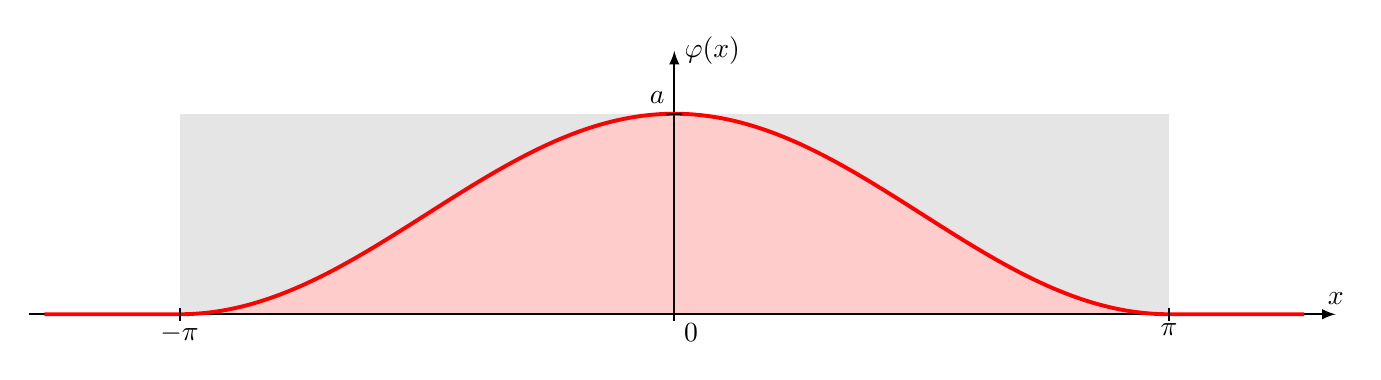
\begin{tikzpicture}[>=latex,xscale=2,yscale=8]
\pgfmathparse{1/3.14159}
\xdef\ip{\pgfmathresult}
\ifthenelse{\boolean{pruefung}}{}{
\fill[color=gray!20] (-3.14159,0)--(3.14159,0)
		--(3.14159,{\ip})--(-3.14159,{\ip});
}
\fill[color=red!20]
	plot[domain=-180:180,samples=360]
		({3.14159*\x/180},{0.5*\ip*(cos(\x)+1)}) --cycle;
\draw[->,line width=0.7pt] (-4.1,0)--(4.2,0)
	coordinate[label={$x$}];
\draw[->,line width=0.7pt] (0,-0.01)--(0,{\ip+0.1})
	coordinate[label={right:$\varphi(x)$}];
\draw[line width=1.4pt,color=red] (-4,0)
	--
	plot[domain=-180:180,samples=360] ({3.14159*\x/180},{0.5*\ip*(cos(\x)+1)})
	-- (4,0);
\draw[line width=0.7pt] (-3.14159,-0.01)--(-3.14159,0.01);
\node at (-3.14156,0) [below] {$-\pi$};
\draw[line width=0.7pt] (3.14159,-0.01)--(3.14159,0.01);
\node at (3.14156,0) [below] {$\pi$};
\node at (0,{1/3.14156}) [above left] {$a$};
\draw[line width=0.7pt] (-0.05,{1/3.15169})--(0.05,{1/3.141569});
\node at (0,0) [below right] {$0$};
\end{tikzpicture}
\end{figure}

\begin{hinweis}
Versuchen Sie die Teilaufgaben a) und b) zu lösen ohne dass Sie ein
Integral auswerten müssen.
\end{hinweis}

\thema{Wahrscheinlichkeitsdichte}
\thema{Verteilungsfunktion}
\thema{Erwartungswert}
\thema{Varianz}

\begin{loesung}
\begin{teilaufgaben}
\item
Die $\cos$-Kurve ist über den Teilintervallen $[-\pi,0]$ und $[0,\pi]$
jeweils punktsymmetrisch bezüglich der Wendepunkte.
Die Kurve halbiert daher das Rechteck mit den Ecken $(-\pi,0)$, $(\pi,0)$,
$(\pi,a)$ und $(-\pi,a)$.
Das Rechteck hat Flächeninhalt $2\pi a$, daher ist der Flächeninhalt unter
der Kurve genau dann $=1$, d.~h.~erfüllt die Normierungsbedingung 
\[
\int_{-\infty}^\infty \varphi(x)\,dx = 1
\]
für eine Wahrscheinlichkeitsdichte, wenn $\pi a=1$ oder
$a=\frac1{\pi}=0.318309886$.
\item
Weil $\varphi(x)$ eine gerade Funktion ist, ist $E(X)=0$.
\item 
Für die Varianz muss man $E(X^2)$, bestimmen, es ist nämlich
$\operatorname{var}(X)=E(X^2)-E(X)^2 = E(X^2)$.
\begin{align*}
E(X^2)
&=
\int_{-\infty}^\infty x^2 \varphi(x)\,dx
=
\frac1{2\pi}
\int_{-\pi}^{\pi}
x^2 (1+\cos x)\,dx
\\
&=\frac{\pi^2-6}{3}
=
1.2898681
\qedhere
\end{align*}
\end{teilaufgaben}
%(%i1) integrate(x^2 * (1/2) * (1 + cos(%pi * x)), x);
%		 2  2					        3  3
%	   (3 %pi  x  - 6) sin(%pi x) + 6 %pi x cos(%pi x) + %pi  x
%(%o1) 	   ---------------------------------------------------------
%					 3
%				    6 %pi
%(%i2) integrate(x^2 * (1/2) * (1 + cos(%pi * x)), x, -1, 1);
%				      2
%				   %pi  - 6
%(%o2) 				   --------
%					 2
%				    3 %pi
\end{loesung}

\begin{bewertung}
\begin{teilaufgaben}
\item Normierungskriterium ({\bf N}) 1 Punkt, Wert von $a$ ({\bf A}) 1 Punkt.
\item Integral für Erwartungswet ({\bf I}) 1 Punkt,
Erwartungswert ({\bf E}) 1 Punkt.
\item Varianzformel ({\bf V}) 1 Punkt,
Wert der Varianz ({\bf W}) 1 Punkt.
\end{teilaufgaben}
\end{bewertung}
